\documentclass{ximera}
\input{../preamble.tex}
\title{Orthogonal Projections} \license{CC BY-NC-SA 4.0}

\begin{document}
\begin{abstract}
 \end{abstract}
\maketitle

\begin{onlineOnly}
\section*{Orthogonal Projections}
\end{onlineOnly}

Given a line $l$ and a vector $\vec{v}$ emanating from a point on $l$, it is sometimes convenient to express $\vec{v}$ as the sum of a vector $\vec{v}_{\parallel}$, parallel to $l$, and a vector $\vec{v}_{\perp}$, perpendicular to $l$.  If you have taken a physics course, you may have seen a force vector decomposed into the sum of two components: one parallel and one perpendicular to the direction of motion.

\begin{center}
 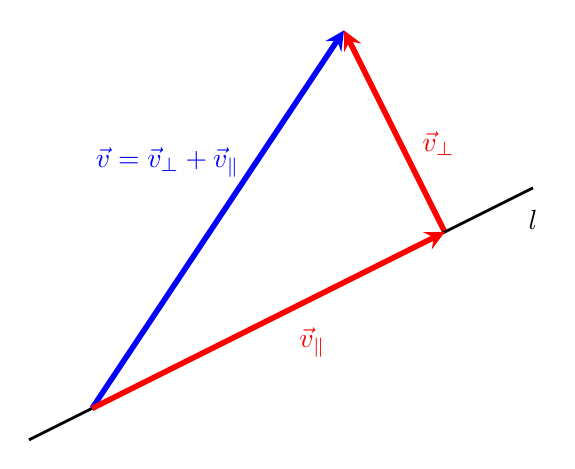
\begin{tikzpicture}[scale=.8]
  \draw[line width=2pt,red,-stealth](3.6, 0.8)--(2,4);
  \node[red] at (3.5, 2.2)   (a) {$\vec{v}_{\perp}$};
 \node[red] at (1.5, -0.95)   (b) {$\vec{v}_{\parallel}$};
  \node[] at (5, 1)   (c) {$l$};
  \node[blue] at (-0.8, 1.9)   (d) {$\vec{v}=\vec{v}_{\perp}+\vec{v}_{\parallel}$};
   \draw [-,line width=1pt]  (-3,-2.5)--(5, 1.5);
\draw[line width=2pt,blue,-stealth](-2, -2)--(2,4);
\draw[line width=2pt,red,-stealth](-2, -2)--(3.6, 0.8);
\end{tikzpicture}

\end{center}

Suppose $\vec{d}$ is a direction vector for $l$.  Then $\vec{v}_
{\parallel}=k\vec{d}$ for some scalar $k$.  Our goal is to find $k$.  
\begin{align*}\vec{v}\dotp\vec{d}&=(\vec{v}_{\parallel}+\vec{v}_{\perp})\dotp\vec{d}\\
&=(k\vec{d}+\vec{v}_{\perp})\dotp\vec{d}\\
&=k\vec{d}\dotp\vec{d}+\vec{v}_{\perp}\dotp\vec{d}\\
&=k\norm{\vec{d}}^2+0\\
&=k\norm{\vec{d}}^2
\end{align*}
We conclude that $$k=\frac{\vec{v}\dotp\vec{d}}{\norm{\vec{d}}^2}$$
and $$\vec{v}_{\parallel}=k\vec{d}=\left(\frac{\vec{v}\dotp\vec{d}}{\norm{\vec{d}}^2}\right)\vec{d}$$

The vector $\vec{v}_{\parallel}=\left(\frac{\vec{v}\dotp\vec{d}}{\norm{\vec{d}}^2}\right)\vec{d}$ is called the \dfn{projection of $\vec{v}$ onto $\vec{d}$}.  In our discussion, $\vec{d}$ is a direction vector for line $l$.  So, we can also say that $\vec{v}_{\parallel}$ is the \dfn{projection of $\vec{v}$ onto $l$}.

To find $\vec{v}_{\perp}$, observe that $\vec{v}_{\perp}=\vec{v}-\vec{v}_{\parallel}$.


\begin{definition}\label{def:projection}
Let $\vec{v}$ be a vector, and let $\vec{d}$ be a non-zero vector.  The \dfn{projection of $\vec{v}$ onto $\vec{d}$} is given by 
$$\mbox{proj}_{\vec{d}}\vec{v}=\left(\frac{\vec{v}\dotp\vec{d}}{\norm{\vec{d}}^2}\right)\vec{d}$$
\end{definition}

\begin{example}\label{ex:projection1}
Find the projection of $\vec{v}$, shown below, onto the line given by $y=\frac{1}{2}x-1$.

\begin{center}
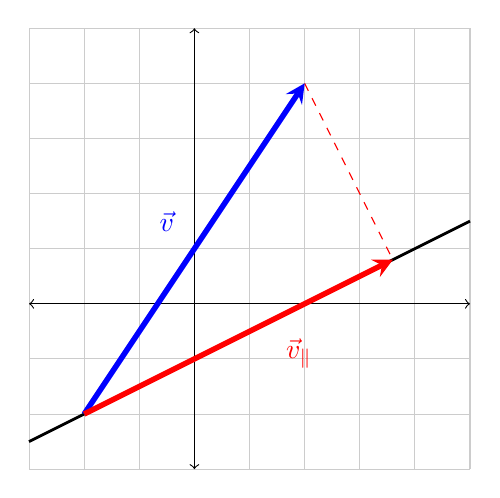
\begin{tikzpicture}[scale=.7]

\draw[thin,gray!40] (-3,-3) grid (5,5);
  \draw[<->] (-3,0)--(5,0);
  \draw[<->] (0,-3)--(0,5);
  \draw[red, dashed] (2,4)--(3.6, 0.8); 
  \draw [-,line width=1pt]  (-3,-2.5)--(5, 1.5);
\draw[line width=2pt,blue,-stealth](-2, -2)--(2,4);
\draw[line width=2pt,red,-stealth](-2, -2)--(3.6, 0.8);
\node[blue] at (-0.5, 1.5)   (a) {$\vec{v}$};
\node[red] at (1.9, -0.9)   (b) {$\vec{v}_{\parallel}$};
\end{tikzpicture}
\end{center}

\begin{explanation}
We begin by finding vectors $\vec{v}$ and $\vec{d}$. The tail of $\vec{v}$ is located at $(-2, -2)$, and the head of $\vec{v}$ is at $(2, 4)$.  Using the ``head-tail" formula we get 
$$\vec{v}=\begin{bmatrix}2-(-2)\\4-(-2)\end{bmatrix}=\begin{bmatrix}4\\6\end{bmatrix}$$ The direction vector for the line $y=\frac{1}{2}x-1$ is $$\vec{d}=\begin{bmatrix}2\\1\end{bmatrix}$$
We find that $\vec{v}\dotp\vec{d}=14$ and $\norm{\vec{d}}^2=5$.
Thus $$\mbox{proj}_{\vec{d}}\vec{v}=\left(\frac{\vec{v}\dotp\vec{d}}{\norm{\vec{d}}^2}\right)\vec{d}=\frac{14}{5}\begin{bmatrix}2\\1\end{bmatrix}=\begin{bmatrix}28/5\\14/5\end{bmatrix}$$
\end{explanation}
\end{example}

\subsection*{A Visual Guide to Creating an Orthogonal Basis}  
Given an arbitrary basis $\{\vec{v}_1, \vec{v}_2\}$ of $\RR^2$, let's start building our orthogonal basis, $\{\vec{f}_1, \vec{f}_2\}$, by setting $\vec{f}_1 = \vec{v}_1$. To find the next element of our orthogonal basis, consider the orthogonal projection of $\vec{v}_2$ onto $\vec{f}_1$.  (See the figure below.)  
\begin{center}
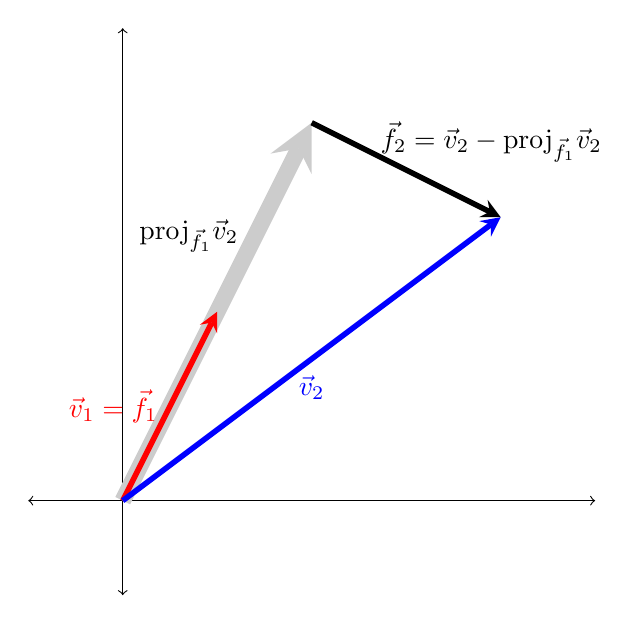
\begin{tikzpicture}[scale=1.2]
 \draw[<->] (-1,0)--(5,0);
  \draw[<->] (0,-1)--(0,5);
  \draw[line width=6pt,-stealth, black!20!white](0,0)--(2,4);
\draw[line width=2pt,red,-stealth](0,0)--(1,2);  
\draw[line width=2pt,blue,-stealth](0,0)--(4,3);
\draw[line width=2pt,-stealth](2,4)--(4,3);  
\node[] at (0.7, 2.8)  (p2)    {$\mbox{proj}_{\vec{f}_1}\vec{v}_2$};
\node[] at (3.9, 3.8)  (p2)    {$\vec{f}_2=\vec{v}_2-\mbox{proj}_{\vec{f}_1}\vec{v}_2$};
\node[red] at (-0.1, 1)  (p2)    {$\vec{v}_1=\vec{f}_1$};
\node[blue] at (2, 1.2)  (p2)    {$\vec{v}_2$};
%\draw[line width=2pt,-stealth](0,0)--(2,-1); 
%\node[] at (1.1, -0.3)  (p2)    {$\vec{f}_2$};
 \end{tikzpicture}
 \quad\quad
\begin{tikzpicture}[scale=1.2]
 \draw[<->] (-1,0)--(5,0);
  \draw[<->] (0,-1)--(0,5);
%  \draw[line width=6pt,-stealth, black!20!white](0,0)--(2,4);
\draw[line width=2pt,red,-stealth](0,0)--(1,2);  
%\draw[line width=2pt,blue,-stealth](0,0)--(4,3);
%\draw[line width=2pt,-stealth](2,4)--(4,3);  
%\node[] at (0.7, 2.8)  (p2)    {$\mbox{proj}_{\vec{v}_1}\vec{v}_2$};
%\node[] at (3.9, 3.8)  (p2)    {$\vec{f}_2=\vec{v}_2-\mbox{proj}_{\vec{f}_1}\vec{v}_2$};
\node[red] at (0.2, 1)  (p2)    {$\vec{f}_1$};
%\node[blue] at (2, 1.2)  (p2)    {$\vec{v}_2$};
\draw[line width=2pt,-stealth](0,0)--(2,-1); 
\node[] at (1.1, -0.3)  (p2)    {$\vec{f}_2$};
 \end{tikzpicture}
\end{center}
Next, let $\vec{f}_2=\vec{v}_2-\mbox{proj}_{\vec{f}_1}\vec{v}_2$.  Observe that $\vec{f}_2$ is orthogonal to $\vec{f}_1$ (See Theorem \ref{th:orthDecompX} of \href{https://ximera.osu.edu/linearalgebradzv3/LinearAlgebraInteractiveIntro/RTH-0010/main}{Orthogonality and Projections}).  This gives us an orthogonal collection $\mathcal{B}=\{\vec{f}_1,\vec{f}_2\}$.  It is intuitively clear that $\vec{f}_1$ and $\vec{f}_2$ are linearly independent.  Therefore $\mathcal{B}$ is an orthogonal basis of $\RR^2$.

The following exploration illustrates this process dynamically.

\begin{exploration}\label{exp:orth1}
Choose an arbitrary basis $\{\vec{v}_1, \vec{v}_2\}$ of $\RR^2$ by dragging the tips of vectors $\vec{v}_1$ and $\vec{v}_2$ to desired positions.  Use the navigation bar at the bottom of the interactive window to go through the steps of constructing an orthogonal basis of $\RR^2$.

\pdfOnly{
Access GeoGebra interactives through the online version of this text at 

\href{https://ximera.osu.edu/linearalgebradzv3/LinearAlgebraInteractiveIntro}{https://ximera.osu.edu/linearalgebradzv3/LinearAlgebraInteractiveIntro}.
}

\begin{onlineOnly}
\begin{center}
\geogebra{xtqppyav}{800}{600}
\end{center}
\end{onlineOnly}
\end{exploration}

We can apply this process to any two-dimensional subset of $\RR^n$.  The following exploration will guide you through the process of constructing an orthogonal basis for a plane spanned by two arbitrary vectors in $\RR^3$.

\begin{exploration}\label{exp:orth2}
Let $W =\mbox{span}\left({\bf v}_1,{\bf v}_2\right)$. $W$ is a plane through the origin in $\RR^3$.  Use the navigation bar at the bottom of the interactive window to go through the steps of constructing an orthogonal basis for $W$.  RIGHT-CLICK and DRAG to rotate the image for a better view.

\pdfOnly{
Access GeoGebra interactives through the online version of this text at 

\href{https://ximera.osu.edu/linearalgebradzv3/LinearAlgebraInteractiveIntro}{https://ximera.osu.edu/linearalgebradzv3/LinearAlgebraInteractiveIntro}.
}

\begin{onlineOnly}
    \begin{center}
\geogebra{zghsfkym}{900}{600}
\end{center}
\end{onlineOnly}
\end{exploration}

In the next exploration, we take the process of constructing an orthogonal basis to the edge of the visual realm and construct an orthogonal basis for $\RR^3$.

\begin{exploration}\label{exp:orth3}
In the GeoGebra interactive below $\{\vec{v}_1, \vec{v}_2, \vec{v}_3\}$ is a basis of $\RR^3$.  Use check boxes to go through the steps for constructing an orthogonal basis starting with the given basis.  RIGHT-CLICK and DRAG to rotate the image for a better view.

\pdfOnly{
Access GeoGebra interactives through the online version of this text at 

\href{https://ximera.osu.edu/linearalgebradzv3/LinearAlgebraInteractiveIntro}{https://ximera.osu.edu/linearalgebradzv3/LinearAlgebraInteractiveIntro}.
}

\begin{onlineOnly}
\begin{center}
\geogebra{qjpvmsws}{900}{800}
\end{center}
\end{onlineOnly}
\end{exploration}

What we saw above are low-dimension examples of what is known as \dfn{Gram Schmidt Orthogonalization}.  


\section*{Practice Problems}

  \begin{problem}\label{prob:proj1a}
  Find $\mbox{proj}_{\vec{d}}\vec{v}$ if $\vec{d}=\begin{bmatrix}-1\\3\end{bmatrix}$ and $\vec{v}=\begin{bmatrix}1\\4\end{bmatrix}$.
  $$\mbox{proj}_{\vec{d}}\vec{v}=\begin{bmatrix}\answer{-1.1}\\\answer{3.3}\end{bmatrix}$$
    \end{problem}
    
    \begin{problem}\label{prob:proj1b}
    Find $\mbox{proj}_{\vec{d}}\vec{v}$ if $\vec{d}=\begin{bmatrix}0\\2\\1\end{bmatrix}$ and $\vec{v}=\begin{bmatrix}-1\\-4\\2\end{bmatrix}$.
    $$\mbox{proj}_{\vec{d}}\vec{v}=\begin{bmatrix}\answer{0}\\\answer{-2.4}\\\answer{-1.2}\end{bmatrix}$$
    \end{problem}

    \begin{problem}\label{prob:proj3}
Show that $\mbox{proj}_{\vec{d}}\vec{v}$ does not depend on the length of $\vec{d}$ by proving that $\mbox{proj}_{\vec{d}}\vec{v}=\mbox{proj}_{k\vec{d}}\vec{v}$ for $k\neq 0$.  What does this result mean geometrically?  Illustrate your response with a diagram.
\end{problem}

\begin{problem}\label{prob:proj2}
Find the projection of vector $\vec{v}$ onto line $l$. (If entering answers in decimal form, round to the nearest one hundredth.)

\begin{center}
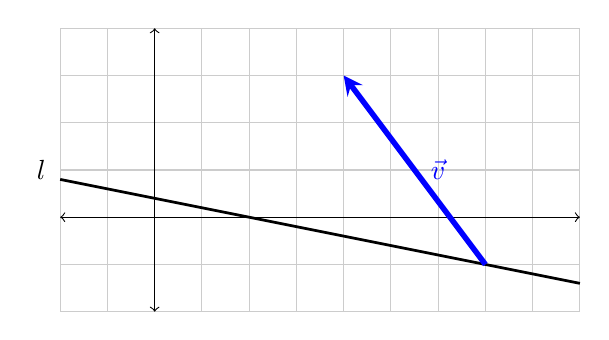
\begin{tikzpicture}[scale=.6]
\draw[thin,gray!40] (-2,-2) grid (9,4);
  \draw[<->] (-2,0)--(9,0);
  \draw[<->] (0,-2)--(0,4);
  \node[blue] at (6, 1)   (a) {$\vec{v}$};
  \node[] at (-2.4, 1)   (b) {$l$};
  \draw [-,line width=1pt]  (-2,0.8)--(9, -1.4);
\draw[line width=2pt,blue,-stealth](7, -1)--(4,3);
\end{tikzpicture}
\end{center}

Answer:
$$\begin{bmatrix}\answer[tolerance=0.005]{-95/26}\\\answer[tolerance=0.005]{19/26}\end{bmatrix}$$
\end{problem}

  

\begin{problem}\label{GS1}
Convert the given basis $\mathcal{B}$ of $\RR^2$ to an orthogonal basis by following the procedure described in this section with $\vec{v}_1=\begin{bmatrix}2\\ 1\end{bmatrix}$.
$$\mathcal{B} = \left\{ \begin{bmatrix}2\\ 1\end{bmatrix}, \begin{bmatrix}1\\ -1\end{bmatrix}\right\}$$

 $$\left\{\begin{bmatrix}2\\1\end{bmatrix},\begin{bmatrix}\answer{-3/5}\\\answer{6/5}\end{bmatrix}\right\}$$

\end{problem}

% \begin{problem}\label{GS2}
% Convert the given basis $\mathcal{B}$ of $\RR^2$ to an orthogonal basis by projecting the first vector onto the second.
% $$\mathcal{B} = \left\{\begin{bmatrix}2\\ 1\end{bmatrix}, \begin{bmatrix}1\\ 2\end{bmatrix}\right\}$$
% \end{problem}

\end{document}
